% Encoding: UTF-8
\documentclass[final,bibliography=totocnumbered]{include/sikseminar}

%% Folgende Pakete werden bereits durch die sikseminar-Klasse geladen:
%\usepackage[german]{babel}
%\usepackage[headsepline]{scrlayer-scrpage}
%\usepackage{german}
%\usepackage{graphicx}
%\usepackage{textcomp}
%\usepackage{bibgerm}

\usepackage[utf8]{inputenc}
\usepackage{todonotes}
\usepackage{hyperref}
\usepackage[T1]{fontenc}
\hypersetup{colorlinks = true,linkcolor = black,citecolor = black,urlcolor = black,filecolor = black}
\usepackage{enumitem}
\usepackage[acronym,toc,section=section,numberedsection,nomain]{glossaries}
\usepackage{paralist}
\glstoctrue
\makeglossaries
\newacronym[shortplural={CPS},longplural={Cyber-physical Systems}]{cps}{CPS}{Cyber-physical System}


\usepackage[autostyle=true,german=quotes]{csquotes}

\graphicspath{{./figure/}}

\usetikzlibrary{shapes.geometric}

\clubpenalty=10000
\widowpenalty=10000


\overfullrule=1mm

\newcommand{\fb}[1]{\dofb#1}
\newcommand{\dofb}[1]{\textbf{#1}\nobreak\hspace{0pt}}


\begin{document}

\Title[Security Considerations for \glsentrytext{cps}]{Security Considerations for Cyber-Physical Systems}
\makeTitle

\Author{Maximilian Ammann}
\Studiengang{Bachelor Informatik}
\makeAuthor
\date{Datum des Vortrags \todo}
\subject{Seminar Cyber-Physical Systems}

\maketitle

\begin{abstract}
\section*{Kurzfassung}
Eine kurze Zusammenfassung der Ausarbeitung mit 10-12 Zeilen Text.
\end{abstract}
\thispagestyle{empty}
\newpage
\tableofcontents
\newpage

\section{Einführung}\label{sec:intro}
% Anforderungen an CPS: Predictability (Lee08)
% Challanges (SGL+08)
% Vision von CPS (RLS+10)
% IoT Constaint: Battery (YWY+17)
\glspl{cps} sind meist eingebettete echtzeit Systeme, welche eine hohe Verfügbarkeit, Robustheit,Widerstandsfähigkeit und Berechenbarkeit aufweisen müssen.
Die physische Welt macht hohe Verfügbarkeit allerdings oft schwierig da sie alles andere als berechenbar ist~\cite{Lee08,SGL+08}.
Einsatzorte für diese Systeme könnten intelligente Stromnetze, symbiotische Sensornetzwerke für die Agrarwirtschaft und Katastrophenabwehr, medizinische oder assistierende Geräte, intelligente Verkehrssteuerung und intelligente Gebäude sein~\cite{RLS+10}.

In all diesen Beispielen spielt ein außerordentliches Maß an Vertrauen eine Rolle~\cite{SGL+08}.
Dieses ist zwar auch bei klassischen Systemen gefordert, allerdings nicht in gleicher Weise, da sie nicht in gleicher Weise an physische Prozesse gekoppelt sind~\cite{BG11}.
Zudem unterliegt man konzeptionell bedingt auch einigen Restriktionen wie beispielsweise die Bindung an eine Batterie oder eine leichte Bauweise~\cite{YWY+17}.
Es existiert also ein Unterschied in den Anforderungen an \glspl{cps} und klassischen Systemen, wie Anwendungsservern oder Heimcomputern, sodass diese beiden in Bezug auf Sicherheit anders betrachtet werden müssen.

In dem Kapitel~\ref{sec:bedeutung-sicherheit} wird zunächst das Zusammenspiel von ''cyber'' und ''physical'' im Bezug auch Sicherheit geklärt.
Zudem werden mögliche Ziele und Angreifergruppen in den Kapitel~\ref{subsec:angriffsziel}~und~\ref{subsec:angreifergruppen} beleuchtet.
Im Kapitel~\ref{sec:angriffszenarien} werden mögliche Szenarien und im Kapitel ~\ref{subsec:angreifergruppen} dazu Gegenmaßnahmen dargestellt.
Zuletzt soll im Kapitel~\ref{sec:diskussion} diskutiert werden ob die genannten Gegenmaßnahmen  für die Szenarien ein adäquate Lösung darstellen.
% Stuxnet (Langer)

% Spectre: https://arxiv.org/pdf/1811.05441.pdf
% EU: https://eur-lex.europa.eu/legal-content/EN/TXT/?uri=JOIN:2017:0450:FIN https://ec.europa.eu/transport/sites/transport/files/3rd-mobility-pack/com20180283_en.pdf


\section{Bedeutung von Sicherheit in \glsentrytext{cps}}\label{sec:bedeutung-sicherheit}
Die Bedeutung von Sicherheit in ''cyber'' Systemen und ''physical'' Systemen unterscheiden sich intrinsisch.
Um Klarheit zu schaffen wo diese Unterschiede liegen soll Sicherheit speziell für \gls{cps} definiert werden.

\subsection{Definition für Sicherheit von \glsentrytext{cps}}\label{subsec:definition}
% CIA triad (Fink) (WYX+10)
% Erweiterung von CIA: Veracity, Plausability (Gollman)
Unter Cybersicherheit versteht man im Allgemeinen Informationssicherheit.
Informationssicherheit kann man durch drei Prinzipien charakterisieren~\cite[,S.~2]{Cherdantseva2013,SFJ2017}:
\begin{itemize}[noitemsep,nolistsep]
\item \fb{Confidentiality} - Nur autorisierte Teilnehmer können auf die Infrastruktur zugreifen.
\item \fb{Integrity} - Die Infrastruktur kann nur von autorisierten Teilnehmer verändert werden.
\item \fb{Availability} - Die Infrastruktur ist für autorisierte Teilnehmer angemessen verfügbar.
\end{itemize}
Zwischen diesen drei Prinzipien muss bei der Entwicklung ein sinnvolles Gleichgewicht gefunden werden.
\citeauthor{GK16} beschreiben, dass bei klassischen Cybersystemen der Fokus auf Confidentiality und bei \glspl{cps} eher auf Availability liegt.
Dieser Fokus ist kritisch zu betrachten, wenn man die diversen Einsatzorte und Anforderungen von \glspl{cps} betrachtet.

Sie schlagen außerdem vor das CIA-Dreieck im Hinblick auf \glspl{cps} durch zwei Prinzipien zu erweitern.
Das erste Prinzip ist Veracity (dt.~Richtigkeit).
Ein System hat diese Eigenschaft genau dann, wenn Aussagen des Systems die Wahrhaftigkeit der vorliegenden Informationen reflektieren.
Es muss also beispielsweise sichergestellt werden, dass Sensoren durch physische Maßnahmen (siehe Kapitel~\ref{subsec:physisch}) geschützt sind.
Confidentiality und Integrity sind nicht ausreichend um die Richtigkeit von Informationen zu garantieren.
Veracity ist eine relativ starke Eigenschaft.
Deshalb kann man in Fällen, in denen diese nur schwer zu erreichen ist, zunächst auf Plausibility setzen.
Herbei hat ein System genau dann diese Eigenschaft, wenn Aussagen des Systems nicht zu weit von erwartbaren Werten abweichen.
Liefert ein Sensor beispielweise einen für physikalische Modelle unmögliche Wert, so ist dieser nicht plausibel und das System erreicht kann einen möglichen Angriff erkennen. \cite{GK16}

\citeauthor{WYX+10} und \citeauthor{SFJ2017} stimmen zu, dass eine Überprüfung auf die Richtigkeit von Informationen wichtig sind.
Sie erweitern das CIA-Dreieck zudem um die Eigenschaft der Authentizität zwischen mehreren Kommunikationspartnern.

Bei \glspl{cps} ist also sowohl die Richtigkeit von Informationen als auch die zweifelsfreie Identifikation zweier Parteien wichtig.
Die Richtigkeit beinhaltet auch, dass es nicht geleugnet werden darf bestimmte Aktionen ausgeführt zu haben \cite{NIST2013}.\todo{Wie zitiert man NIST?}

\begin{figure}
    \centering
    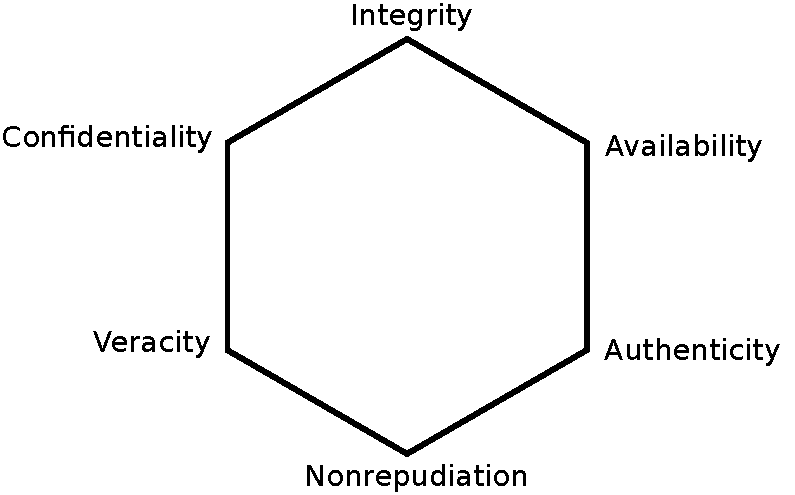
\includegraphics[width=0.5\textwidth]{figure/triad}
    \caption{Erweitertes CIA-Dreieck}
    \label{fig:triad}
\end{figure}

Zusammenfassend kann man sagen, dass die Prinzipien aus der klassische Informationssicherheit nicht ausreichen um das oft komplexe Zusammenspiel von ''physical''- und ''cyber''-Einheiten abzusichern.
Deshalb sind Prinzipien wie Veracity und Authenticity, wie in Abbildung~\ref{fig:triad} zu sehen ust, nötig um die Aspekte von \glspl{cps} abzudecken.

% Definition (BG11)
% computer, information, network, communication, physical security
% Fingerprinting, Network Separation, End System Security (Gollman)


\subsection{\glsentrytext{cps} als Angriffsziel}\label{subsec:angriffsziel}
% (Gollman, 1)
% Survey: medial, IoT, smart grid, power plant (Humayed)
% IoT (FPA+18) (YWY+17)
% Security Considerations in Cloud (SPB+16)


\subsection{Angreifergruppen}\label{subsec:angreifergruppen}
% Cyber-Kriminelle
% Verärgerte Mitarbeiter/Private Gründe
% Terroristen, Aktivisten, kriminelle Gruppen
% Staaten (Cardenas 2009, 2.) (WYX+10, II. C.)

Angriffe können von unterschiedlichen Gruppen aus unterschiedlichen Gründen ausgehen.

% Welche Gruppe? Warum? Auf welche Art? (falls speziell)
\begin{compactenum}[(a)]
    \item Kriminelle Gruppen haben oft Erpressung als Ziel \cite{CAS+09,WYX+10}.
    Dabei sind Cyberangriffe nur ein logischer nächster Schritt der Kriminellen, da diese weitaus günstiger, weniger riskant, nicht durch Entfernungen eingeschränkt und einfacher zu koordinieren und wiederholen sind \cite{CAS+09}.
    \item Erfahrene Forensiker/Hacker haben nicht unbedingt als Ziel selbst ein System zu beschädigen.
    Dabei gibt es zwei Gründe für die Entwicklung von Schadsoftware.
    Zum einen können diese an beispielsweise Staaten verkauft werden (siehe dazu (\ref{group:staaten})). \todo{Zitat fehlt}
    Zum anderen kann die Entwicklung aber auch als Ziel haben die Lücken unter bestimmten Auflagen offen zulegen um diese zu schließen. \todo{Zitat fehlt}
    \item Unzufriedene (ehemalige) Mitarbeiter eines Unternehmens haben viel Wissen über dessen Infrastruktur.
    Zudem existiert eventuell schon oder noch Zugriff auf das System, sodass überhaupt kein Umgehen von Sicherheitsmechanismen notwendig ist. \cite{CAS+09,WYX+10}
    \item Aktivistische Gruppierungen zielen oft auf kritische \glspl{cps}, wie beispielsweise Kernkraftwerke oder \gls{scada} Systemen in Fabriken, ab, um diese zu manipulieren \cite{CAS+09,WYX+10}. \todo{Spionage?}
    Damit dies erreicht werden kann existiert die Möglichkeit erfahrene Forensiker/Hacker oder Insider einzusetzen \cite{WYX+10}.
    % Terroristisch
    \item Staaten können militärisches Interesse daran haben Infrastruktur innerhalb oder außerhalb des Staatsgebiets anzugreifen \cite{CAS+09}, um diese zu zu sabotieren oder auszuspionieren.
    Auch hier werden erfahrene Forensiker/Hacker oder Insider eingesetzt.
    \label{group:staaten}
\end{compactenum}

Das Wissen über den Angreifer und dessen Motivation kann maßgeblich bei der Wahl und der Strategie der Gegenmaßnahmen helfen.
Zudem können Gefahrenmodelle und detailliertere Angriffsszenarien entworfen werden.


\section{Angriffsszenarien}\label{sec:angriffszenarien}
% Sabotage und Spionage
% Punkte wo angegriffen werden kann (Fink, Figure 1.1) (Cardenas 2008, Figure 3)
% Migration von Legacy Systemen ist kritisch (Gollman, 1.)
\subsection{Unterschiede zu klassische Szenarien}\label{subsec:klassisch}
% Unterschied zu klassischen Systemen (Cardenas 2008, 3.)
% IoT Unterschiede zu klassischem (FPA+18)
% Workflow von CPS (WYX+10, II.)
\subsection{Denial-of-Service Angriff}\label{subsec:dos}
% (WYX+10, II. B.)
% (Cardenas 2008, 2.1)
\subsection{Man-in-the-Middle Angriff}\label{subsec:mitm}
% (WYX+10, II. B.)
\subsection{T\"auschungsangriff (Deception)}\label{subsec:tauschung} % Deception
% (Cardenas 2008, 2.1)
\subsection{Lauschangriff (Eavesdropping)}\label{subsec:lauschen} % Eavesdropping
% (WYX+10, II. B.)
\subsection{Compromised-Key Angriff}\label{subsec:key}
% (WYX+10, II. B.)


\section{Gegenmaßnahmen}\label{sec:gegenmassnahmen}
% Properties: Safety, Security, Reliability, Resilence (LLZ+14)

% Least Privilege (Gollman)
% Need-to-Know (Gollman)
% Separation (Gollman)

% Proactive Mechanisms, Reactive Mechanisms, Design and Analysis Principles (Cardenas 2008)

% Context Aware Security: Sensing, Cyber, Control, Physical Security (WYX+10)

\subsection{Modellierung von \glsentrytext{cps}}\label{subsec:modellierung}
% Argument: Neue Grundlage für Embedded Systems/CPS: Modelbasiert anstatt Programm (Lee08)
Noch nicht sicher.

Um hierbei dem Standard an Sicherheit zu genügen schlägt \citeauthor{Lee08} sogar vor eine neue Grundlage für diese Systeme zu etablieren~\cite{Lee08}.

\subsection{Physische Maßnahmen}\label{subsec:physisch}
% (Cardenas)

\subsection{Organisatorische Maßnahmen}\label{subsec:orga}
% Transdiszipliär (Brazell14)
% Betriebsblindheit (Gollman)

\subsection{Präventive Maßnahmen}\label{subsec:präventiv}
% Security by Obscurity (Scarfone2008)
% (Cardenas 2009, 4.)

\subsection{Detektion und Wiederherstellung (Detection and Recovery)}\label{subsec:detektion}
% (Cardenas 2009, 4.)

\subsection{Widerstandsfähigkeit (Resilience)}\label{subsec:widerstand} % Resilience
% (Cardenas 2009, 4.)

% End-to-End Security (Fink)

\subsection{Abschreckung (Deterrence)}\label{subsec:abschreckung} % Deterrence
% (Cardenas 2009, 4.)

\section{Sind die Gegenmaßnahmen für potenzielle Szenarien ausreichen?}\label{sec:diskussion}

Sind sie Notwendig?
Ja! -> Sind sie Ausreichend?

\newpage
\printglossary[type=\acronymtype]
~\nocite{*}

\printbibliography
\newpage
% \listoftodos
\end{document}
